\documentclass{beamer}

\usepackage{beamerthemetuw}
\usepackage{enumitem}
\setbeamercovered{transparent}


\title{Rust Ecosystem}
\subtitle{Adoption, Tooling, Community and Governance}
\author{Florian Sextl, Mark Chimes, Adrian Rebola-Pardo}
\date{\today}

\begin{document}

\begin{frame}
    \titlepage
\end{frame}

\begin{frame}{Outline}
\tableofcontents
\end{frame}

\section{Adoption, Popularity, and Community}
%\sectionpage

%\begin{frame}{Rust in Production - Do You Use Rust Code?} 
%\begin{block}{}
%\begin{itemize} 
%	\item \textbf{Firefox} 
%	12\% of code. Migrated server push-notification architecture.
%	\item \textbf{Rust-For-Linux Project} 
%	Comprises 0.125\% (1/800th) of Linux kernel
%	\item \textbf{Ripgrep} 
%	Powers text search in VS Code
%	\item \textbf{Dropbox}
%	components of core file-storage system
%	\item \textbf{Cloudflare}
%	HTTP proxy (Pingora), DNS stack, DDoS 
%	\item \textbf{AWS}
%	Firecracker virtualization tech
%	\item \textbf{Git} Added first Rust code a few days ago: 
%	libgit-sys and libgit wrappers, and Rust Foreign-Language Interface
%	\item \textbf{Ubuntu} plans to replace GNU utilities with Rust implementations
%	(e.g. \texttt{ls, cp, find, diff})
%\end{itemize} 
%\end{block}
%\end{frame} 

\begin{frame}{Rust in Production - Do You Use Rust Code?} 
\begin{block}{}

\begin{itemize} 
	\item<2-> \textbf{Firefox} 
	12\% of code. Migrated server push-notification architecture.
	\item<3-> \textbf{Rust-For-Linux Project} 
	Comprises 0.125\% (1/800th) of Linux kernel
	\item<4-> \textbf{Ripgrep} 
	Powers text search in VS Code
	\item<5-> \textbf{Dropbox}
	components of core file-storage system
	\item<6-> \textbf{Cloudflare}
	HTTP proxy (Pingora), DNS stack, DDoS 
	\item<7-> \textbf{AWS}
	Firecracker virtualization tech
	\item<8-> \textbf{Git} Added first Rust code a few days ago: 
	libgit-sys and libgit wrappers, and Rust Foreign-Language Interface
	\item<9-> \textbf{Ubuntu} plans to replace GNU utilities with Rust implementations
	(e.g. \texttt{ls, cp, find, diff})
\end{itemize} 
\end{block}
\end{frame}  


\begin{frame}{} 
\begin{center}
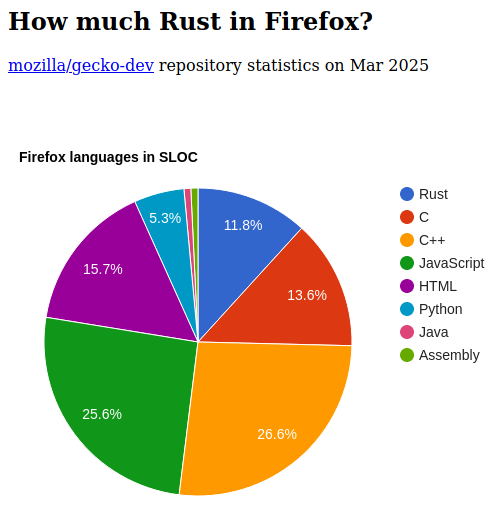
\includegraphics[scale=0.45]{rust-in-firefox}
\end{center}
\url{https://4e6.github.io/firefox-lang-stats/}
\end{frame} 

\begin{frame}{Openhub Rust Language Statistics} 

\begin{center}
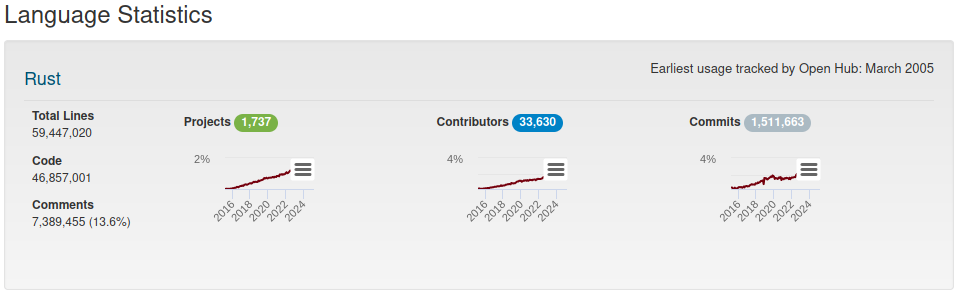
\includegraphics[scale=0.4]{openhub-statistics}
\end{center}

\url{https://openhub.net/languages/rust}


\url{https://madnight.github.io/githut/\#/pull_requests/2024/1}
(next page)

\end{frame} 

\begin{frame}{GitHut 2.0 - Github Language Stats } 
\begin{center}
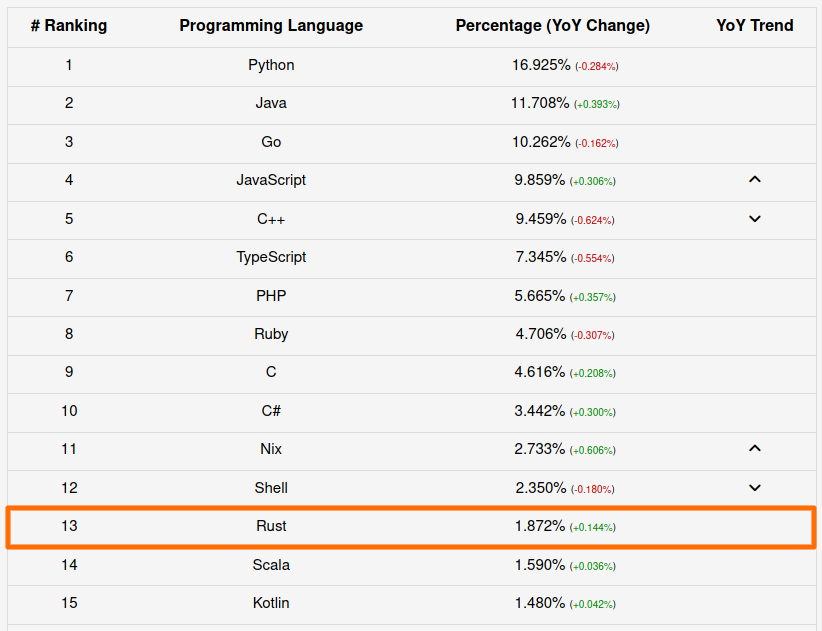
\includegraphics[scale=0.4]{githut-statistics}
\end{center}
\end{frame} 


\begin{frame}{Very Popular With Programmers} 

	\begin{block}{Stack Overflow Survey}

   	Rust is most ``admired", and 6th-most ``desired"

   \end{block}


    \begin{itemize}
    \item \textbf{Admired:} Already use, want to keep using
    \item \textbf{Desired:} Don't use yet, but want to
    \end{itemize} 
    
\end{frame} 

\begin{frame}{Popularity 2023} 
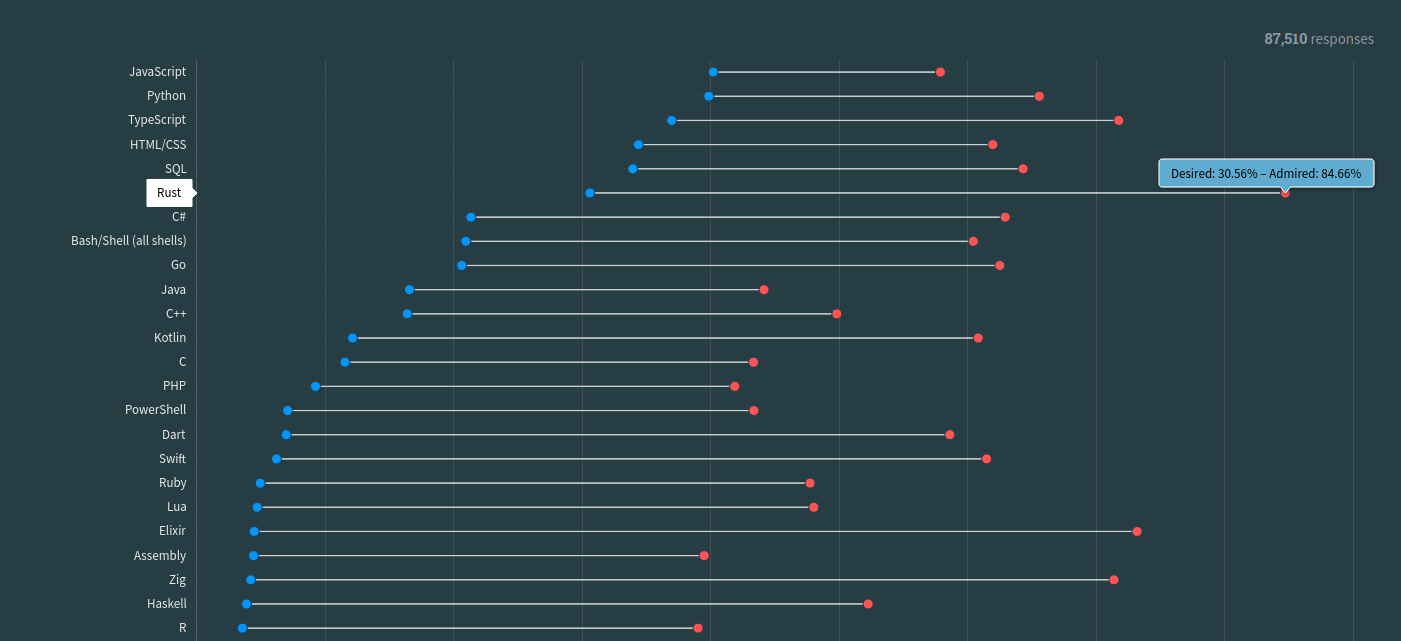
\includegraphics[scale=0.2]{desired-admired-2023}
Admired: 85\%
Desired: 31\%\\
\end{frame} 

\begin{frame}{Popularity 2024} 
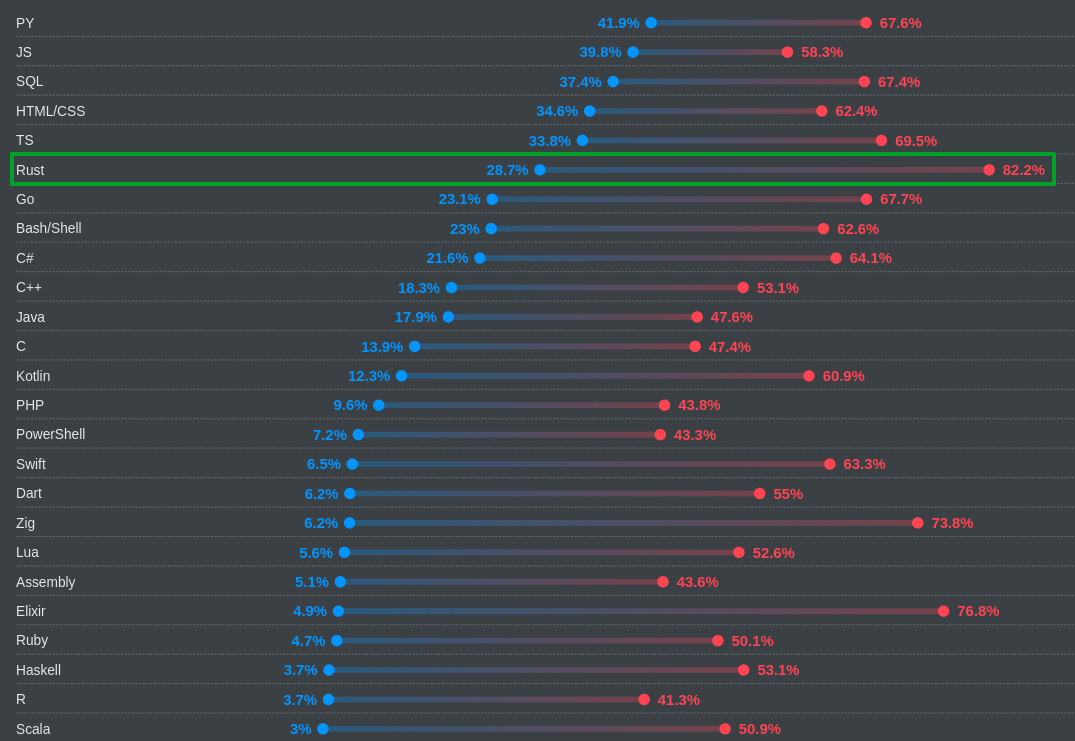
\includegraphics[scale=0.35]{desired-admired-2024}
\end{frame} 


\begin{frame}{Community} 
\begin{block}{}
\begin{quote}
``This is by far the least toxic, most engaging and the nicest dev community I've EVER seen."
\end{quote}
\end{block}
- Reddit user \emph{u/hussainsonreddit} on the Rust subreddit\footnote{\url{https://www.reddit.com/r/rust/comments/ofoi4l/best_developer_community_ive_seen/}}
\end{frame}



\begin{frame}{Community} 
\begin{block}{Rust enthusiasts are ``Rustaceans"}
\begin{itemize}[label=$\bullet$] 
\item Official Rust forums
\item Discord
\item Zulip
\item Reddit
\end{itemize}
\end{block}
\begin{center}

\includegraphics[scale=0.1]{cuddlyferris}

Ferris, the Unofficial Rust Mascot
\end{center}
\end{frame}


\begin{frame}{Others Interested in Rust}
\pause
\begin{block}{Politically} 
February 2024, United States White House issued a report urging that all programmers move to memory-safe programming; mentions Rust by name.
\end{block} 
\pause
\begin{block}{Commercially} 
November 2024, Amazon issued challenge to formally verify safety of Rust standard library
\end{block}
\pause
\begin{block}{Academia} 
Interesting academically: RustBelt project, modelling memory with separation logic, 
Stacked Borrows and Tree Borrows aliasing models...
\end{block} 
\end{frame} 

\section{Tooling and Compilation} 
%\sectionpage
%\begin{frame}{Rust Tooling and Compilation} 
%\begin{center}
%How does it \emph{feel} to use Rust in practice, compared to other programming languages? 
%\end{center}
%\end{frame} \section{Adoption and Popularity}


\begin{frame}{Standard Tooling} 
\vspace{-3em}
\begin{block}
{Basic functionality included by default}
\begin{itemize} [label=$\bullet$] 
\item<2-> compilation \& build files
\item<3-> tests
\item<4-> dependency \& versioning management
\item<5-> documentation generation
\end{itemize}
\end{block}

\pause \pause \pause \pause \pause 
Compare to Python dependency hell: \\
pip, pip-tools, wheel, pyenv, conda, asdf, venv, virtualenv, pipenv, poetry, pypi, flit, conda-forge, anaconda-repo \ldots
\end{frame} 

%\begin{frame}{Basic Tools} 
%\begin{block}{}
%\begin{tabular}{@{}l l@{}}
%\textbf{rustc}        & The compiler \\
%\textbf{Cargo}        & Downloads dependencies, compiles packages, 
%\\ & uploads packages, and makes distributables\\
%\textbf{crates.io}    & Package registry \\
%\textbf{rustup}       & Installs toolchain and manages compiler versions \\
%\end{tabular}
%\end{block}
%\end{frame}

\begin{frame}{Basic Tools} 
\begin{block}{}
\pause 
\begin{tabular}{@{}l l@{}}
\textbf{rustc}        & The compiler \\ \pause
\textbf{Cargo}        & Downloads dependencies, compiles packages, \\ 
                      & uploads packages, and makes distributables\\ \pause
\textbf{crates.io}    & Package registry \\ \pause
\textbf{rustup}       & Installs toolchain and manages compiler versions \\
\end{tabular}
\end{block}
\end{frame}


\begin{frame}{Getting Started: Running Rustup} 
This installs Rustup, Cargo, the Rust compiler etc. Easy! 
\pause 
\begin{block}{$\geq$ Debian 13 (trixie), Ubuntu 24.04 (noble)}
\texttt{sudo apt install rustup}
\end{block}
\pause 
\begin{block}{Other Linux / Mac}
\texttt{curl --proto `=https' --tlsv1.2 -sSf https://sh.rustup.rs | sh}
\end{block}
\pause 
\begin{block}{Windows}
Download and run rustup-init.exe (Also requires installing Visual Studio for linker and Windows API)
\end{block}
\end{frame}

\begin{frame}{Example Cargo Commands} 
\begin{block}{}
\pause
\begin{tabular}{@{}l l@{}}
\texttt{cargo new}     & Create a new Rust project \\ \pause
\texttt{cargo run}     & Build and run \\ \pause
\texttt{cargo build}     & Build without running \\ \pause
\texttt{cargo test}    & Run tests \\ \pause
\texttt{cargo update}  & Update dependencies\\
\end{tabular}
\end{block}
 \pause
Also many useful flags:
\begin{block}{}
\texttt{cargo build --release} \hspace{3em} Build optimized version
\end{block}
\end{frame}

\begin{frame}{Other Tooling} 
\begin{block}{Rust Tools}
\pause 

\begin{tabular}{@{}l l@{}}
\textbf{rust-analyzer}     &  language server (e.g. VS Code plugin) \\ \pause
\textbf{clippy}     &  Linter (correctness, suspicious, style, \\
					&			complexity, performance) \\ \pause
\textbf{Rustfmt}    & auto-format code \\ \pause
\textbf{MIRI}    	& Analyze unsafe code \\ \pause
\textbf{rustdoc}  & Autogenerate documentation (HTML, CSS, \\
					&			and JavaScript)\\ \pause
\textbf{cargo publish} & upload package to crates.io \\
\end{tabular}
\end{block}
\end{frame}



\begin{frame}{Compilation Times} 
\pause 
Common criticism of Rust is compilation times. \pause

Much of this criticism is older; lots of improvement made \pause

Usual causes: Monomorphization, Re-compilation, Detailed compiler error messages \pause

What can you do to speed things up?\\ compilation flags: incremental, opt-level
\pause

Still improving

\end{frame}


\begin{frame}{Compiler Development} 
\begin{itemize} [label=$\bullet$] 
\item<2-> 
Rust has a very strict stability policy and releases every six weeks. (Run
\texttt{rustup update} to update)
\item<3-> 
Many features only available on \emph{nightly} toolchain
\item<4-> 
Each major decision in Rust starts as Request for Comments (RFC).
\end{itemize} 
\end{frame} 


\section{Governance, Licensing, and History} 
%\sectionpage




\begin{frame}{Governance} 

\url{https://github.com/rust-lang/rfcs/blob/master/text/1068-rust-governance.md}
\begin{block}{}
Rust is governed by a core team, [which]:
\begin{itemize} [label=$\bullet$] 
\item    Sets the overall direction and vision for the project;
\item    Sets the priorities and release schedule;
\item    Makes final decisions on RFCs.
\end{itemize}
\end{block}
\end{frame} 



\begin{frame}{Licensing} 
Open source, very permissive licenses.


\begin{block}{Rust Programming Language and official projects}
\begin{itemize}[label=$\bullet$] 
\item
Apache License, Version 2.
\item
MIT license
\end{itemize}
\end{block}


\end{frame}

\begin{frame}{Image Licensing} 

Rust and Cargo logos are owned by Mozilla and distributed under the terms of the Creative Commons Attribution license  \url{https://creativecommons.org/licenses/by/4.0/}
\begin{center}

\includegraphics[scale=0.4]{rust-logo-256x256}

\includegraphics[scale=0.4]{Cargo-Logo-Small}
\end{center}
\end{frame} 




\begin{frame}{History}
    \begin{itemize}
        \item[2006]<2-> Personal project by \textbf{Graydon Hoare} working at Mozilla
        \item[2009]<3-> Officially sponsored by Mozilla
        \item[2013]<4-> Hoare steps down, Rust Core Team formed
        \item[2014]<5-> Request for Comments (RFC) process introduced
        \item[2015]<6-> Rust 1.0 released
        \item[2016]<7-> Rust Mid-Level Intermediate Language (MIR) introduced
        \item[2022]<8-> Supported in Linux Kernel
        \item[2024]<9-> First Linux (network) drivers written in Rust accepted
	\end{itemize}
\end{frame}

\begin{frame} {Fun Fact}
\begin{block}{}
Rust is named after the group of fungal plant pathogens, which Hoare calls “over-engineered for survival.”
\end{block}
\begin{center} 
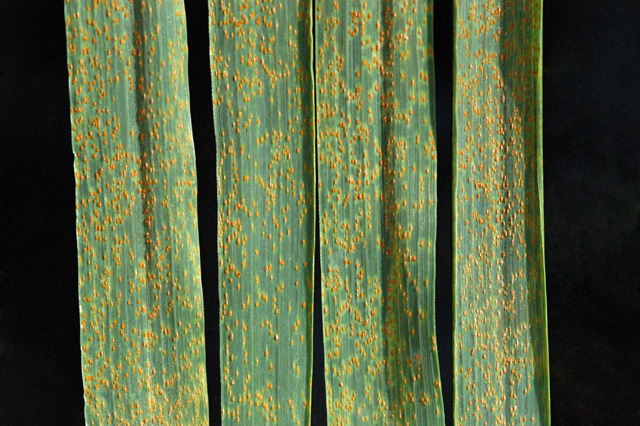
\includegraphics[scale=0.3]{Wheat_leaf_rust_on_wheat}
\end{center}
\end{frame} 


\section{Extra Notes} 
\sectionpage




\begin{frame}{C and Rust Interop} 
Can you call C code from Rust? Yes! 

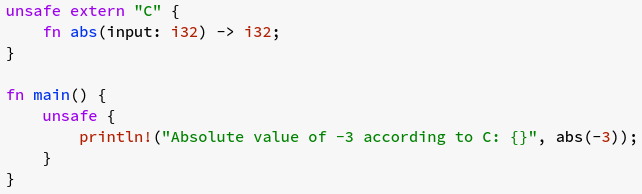
\includegraphics[scale=0.4]{calling-external}

\url{https://doc.rust-lang.org/book/ch20-01-unsafe-rust.html} 

(Requires creating foreign-function-interface (FFI), 
wrapping the exposed C API for use with Rust, converting types, and pre-compiling the C code)
\end{frame} 

\begin{frame}{Rust Verification}
    \begin{itemize}
        \item \textbf{Verified-Rust Tools:}
        \begin{itemize}
            \item \href{https://github.com/verus-lang/verus}{Verus}: Verified Rust for low-level systems code
            \item \href{https://github.com/flux-rs/flux}{Flux}: Refinement Types for Rust
            \item \href{https://github.com/viperproject/prusti-dev}{Prusti}: Static verifier for Rust (Viper-based)
            \item \href{https://github.com/dafny-lang/dafny/issues/5561}{Dafny-Rust Compiler}: Experimental, partial support
        \end{itemize}
        \item \textbf{Creusot:} Automated proof of code correctness
        \begin{itemize}
            \item CreuSAT: Verified SAT solver written in Rust and verified with Creusot
        \end{itemize}
    \end{itemize}
 \end{frame}
        
   \begin{frame}{Rust Verification}
    \begin{itemize}     
        \item \textbf{Aeneas:} Translates MIR to functional Coq/F*
        \item \textbf{Kani:} Model checking
        \item \textbf{Property-Based Testing:}
        \begin{itemize}
            \item \href{https://github.com/BurntSushi/quickcheck}{QuickCheck}: Automated property testing
            \item \href{https://github.com/proptest-rs/proptest}{Proptest}: Hypothesis-like property testing
        \end{itemize}
        \item \textbf{Gilian Rust:} Hybrid approach to semi-automated Rust verification
    \end{itemize}
\end{frame}

\end{document}
